\documentclass[letterpaper,twocolumn,10pt]{article}
\usepackage{usenix2019_v3}

% \usepackage{url}
\PassOptionsToPackage{hyphens}{url}\usepackage{hyperref}
% \usepackage{titlesec}
% \titlespacing*{\section}{0pt}{1.1\baselineskip}{\baselineskip}
\usepackage{tikz}
\usepackage{stfloats}
\usepackage{amsmath}
\usepackage{makecell,xspace}
\usepackage{tabularx}
\usepackage{multirow}
\usepackage{algorithm}
\usepackage{subcaption}
\usepackage{comment}
\usepackage[noend]{algpseudocode}
\usepackage{graphicx}
\usepackage{listings,xcolor}
\usepackage{csvsimple}
\usepackage{adjustbox}
\lstset{numbers=left,numberstyle=\color{red},stepnumber=1,breaklines=true,basicstyle=\tiny\ttfamily,numbersep=0.1pt,columns=fullflexible,moredelim=**[is][\color{blue}]{@}{@}}
\graphicspath{{figures/}}
\newcolumntype{L}{>{\raggedright\arraybackslash}X}

\newcommand{\yuchen}[1]{\textbf{\color{red} Yuchen: #1}}
\newcommand{\sysname}{FastFocus\xspace}

%\renewcommand{\yuchen}[1]{}

\begin{document}
%-------------------------------------------------------------------------------

%don't want date printed
\date{}

% make title bold and 14 pt font (Latex default is non-bold, 16 pt)
\title{\Large \bf \sysname: Camera Focus Speedup with Available Hardware}

%for single author (just remove % characters)
\author{
{\rm Yuchen Yang}\\
Brown University
}

\maketitle

\begin{abstract}

Focusing is a fundamental step for taking pictures.
With currently available hardware in phones and existing focusing methods, it takes longer time to take pictures, especially when we need a large number of photos or faster photo delivery.
The current process does not consider the exact condition of the phones and the camera configurations they have.
Thus we present \sysname, a brandnew mechanism for faster focusing and image capturing which takes less time on both photo capturing and focus evaluation.
It collects the photos at specific focus positions in advance and then picks the most well-focused one as the result.
This saves time from traditional hill climbing by taking fewer pictures and calculates the focus function fewer times.
According to our experiments, \sysname has the average of 2.89s for collecting a well-focused photo, which is 39.7\% faster than hill climbing and the quality loss calculated from Laplacian focus function is less than 18\% in all cases.
\end{abstract}

\vspace{-1em}
\section{Introduction}

People care a lot about the capability of phone cameras and we still have problems while taking photos using phones.
Phone cameras of most brands these days are still limited by the basic cost and the size.~\cite{autofocus}
Some new types of phones from Apple, Samsung, LG and Google Pixel are using new methods like phase contrast and laser detection to get a more accurate distance between the camera and the object.
These methods surely improves the speed of focusing while capturing photos, at the cost of better hardware and potential slight errors.

Most phones still use traditional cameras, which includes a motor for lens group moves and hill climbing (trial-and-error) for focusing.
The lens group starts from a position, moving towards one direction at a large step and compare the focusing effect with the previous capture.
Once the photo quality decreases, the lens group moves towards the reverse direction, with a smaller step, until the step is at the minimum.

There are many previous works discussing how we should tell a photo is well-focused.
These focus functions mostly are based on derivatives, which directly show how sharp an edge is.
This indicates whether a photo is clear and not blurred.
Some methods pick all the pixels of the photo and sum up the derivatives at each pixels as the final value for focus evaluation.
Other methods pick only part of them and choose the orientation of the picked pixels respectively.

The traditional hardware and methods indicate that the speed of focusing is always slow but the outcome is fairly good.
However, there are problems when we need to speed up the photographing process, especially when we need to collect a large amount of photos or quickly collect most photos at a relatively fixed distance.
To save some time, we present \sysname as a brandnew solution, which greatly improves the photo capturing speed while the photo quality loss is little.

Our design is pretty simple.
Instead of having the lens group moving back and forth several rounds, we move in only 1 direction, collect all the photos at a larger step.
The step value should be smaller than the starting step of hill climbing but slightly larger than the minimal step in hill climbing.
This way, we may lose the accuray to some extent, but we save time by taking fewer photos and calculating focus function fewer times as well.

We implement our own version of hill climbing and 2 new versions of \sysname, all in Python.
We collect 5 groups of photos as the input for the 3 algorithms.
The object distance of these groups range from 5 centimeters to 1 meter.
The results show that v1 of \sysname has a slightly faster speed than traditional hill climbing and surprisingly better focus effect in some cases.
v2 of \sysname has much faster focusing speed with a boost up to 50.3\% and 39.7\% on average.
The quality loss is pretty low, which is less than 18\% in the worst case and 8.1\% on average.

\section{Background}

We usually experience the following steps when trying to get a well-focused photo:
\begin{enumerate}
	\item Get the image with the camera when the lens group is at the current position.
	\item Evaluate whether the image is blurred and get a value using the focus function.
	\item Compare the value with the previous value. If the value grows larger (image gets better focused), the current moving direction is correct.
	\item Move the lens group towards the direction.
	\item Repeat the process until the value gets smaller or the evaluated value cannot be further improved.
\end{enumerate}

During this process, we need to decide the focusing method we use, the focus function, how we move the lens group and the specifications of the camera we use.
Now we introduce the parts one by one.

\subsection{Existing Focusing Methods}
There are mainly three categories of focusing methods in current phones~\cite{autofocus}.

\textbf{Contrast Detection} is the standard and traditional method we use in most phones.
It applies trial and error.
The lens group move back and forth until the position of the maimum focus function value is found.
This method is slow and takes time to move the lens and evaluate the autofocus effects.
However, the outcome figures are fairly good in most cases, except for low-light conditions.

\begin{figure}[tb!]
	\begin{center}
		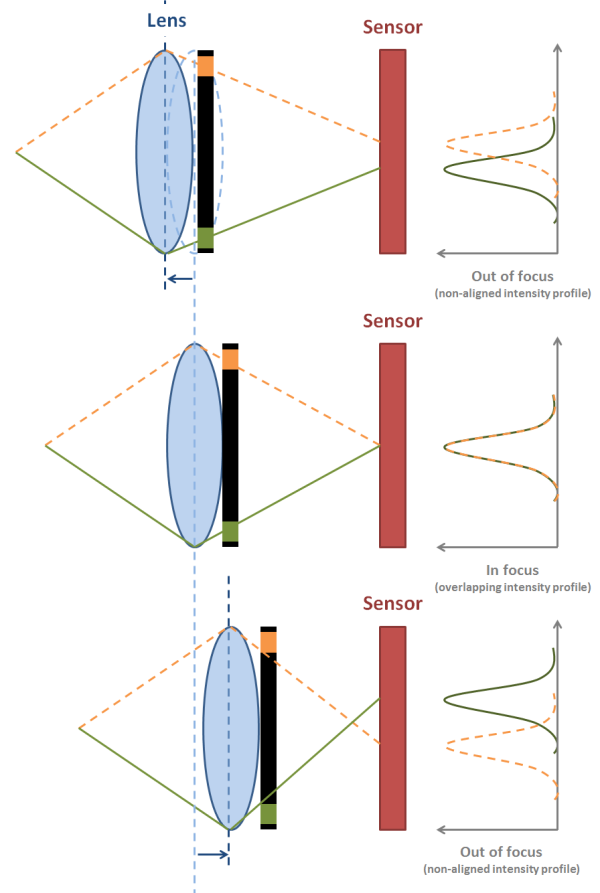
\includegraphics[width=2in]{phasedetection}
	\end{center}
	\caption{Basic ideas of phase detection}
	\label{f:phasedetection}
\end{figure}

\textbf{Phase Detection} is a better method which requires more expensive hardware.
This technique is usually applied in digital single-lens reflex cameras.
As shown in Figure~\ref{f:phasedetection}, there are 2 apertures on opposite sides of the lens and they leave 2 light rays which provides different intensity profile if they are not well focused.
The system can thus decide exactly how much the lens need to be adjusted according to the profiles.
This is much faster but requires better hardware and still suffers in low-light conditions.

\textbf{Laser detection} is a method similar to Radar and calculates the time for the laser to be reflected.
It is super fast and works in low-light conditions as well.
However, it is effective only in short distances and may be biased by transparent objects like windows.

\subsection{Focus Functions}

Focus functions are methods to evaluate whether a picture is well-focused.
In general, the functions include calculating sharpness difference with neighboring points for some sampling pixels or all pixels in the picture.

There are quite some papers explaining different focus functions~\cite{focusfunction}.
In general, there are 4 types based on derivatives, statistics, histograms and intuitive.
Statistics-based methods use variance or correlation of all the pixels.
Hisograms-based methods summarize the histogram of grey-level intensities of pixels and calculates the range or entopy.
Intuitive-based methods sums up the intensities above the threshold as the function.
These 3 types of methods above are less popular than derivative-based methods.
Here the derivative could be absolute difference, square, Laplacian operator, Sobel operator, etc.
Different methods have slightly different effect for various scenarios.

In our implementation, we use existing Python library and applies Laplacian operator.

\subsection{Hill Climbing}

Hill climbing is basicly trial-and-error.
We usually have a function $y=F(x)$ and a range for $x$.
We hope to find the maximum value of $y$ among the range of $x$.

$x$ starts from one edge of the range, select a basic step, and keep moving towards the other end at the interval of the step.
Every time when $x$ changes, we calculate the $y$ value and if $y$ increases, we keep move $x$ towards the same direction.
Otherwise, we reduce the step size and move $x$ towards the opposite direction.
This keeps going until the $y$ value cannot be further increased.

\begin{figure}[tb!]
	\begin{center}
		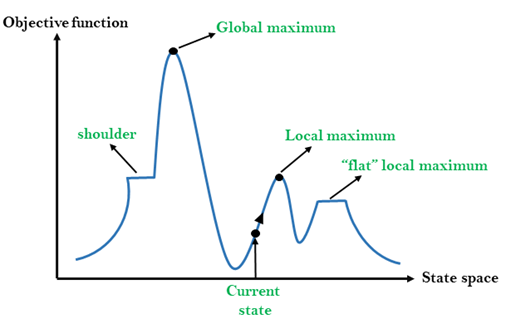
\includegraphics[width=2in]{hillclimb}
	\end{center}
	\caption{Example of traditional hill climbing}
	\label{f:hillclimb}
\end{figure}

As shown in Figure~\ref{f:hillclimb}, we can see that there are 1 global maximum and multiple local maximum.
Only using the method mentioned above, we may fall into local maximum and not get the best value.
Simulated annealing and random walks may help with the situation and lead us to global maximum.

\subsection{Camera Specifications}

\begin{figure}[tb!]
	\begin{center}
		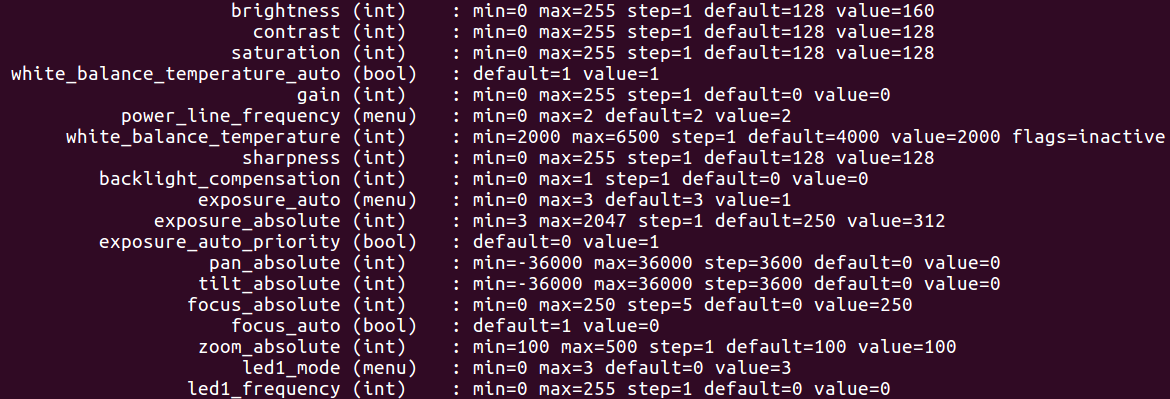
\includegraphics[width=3in]{param}
	\end{center}
	\caption{Controllable camera parameters}
	\label{f:param}
\end{figure}

We use Logitech C920 for the experiments.
This is a camera which follows UVC (USB video device class standard) and it can be controlled by v4l2 tool.
All the available parameters are listed in Figure~\ref{f:param}.

Among all the parameters, we care about focus\_absolute the most.
focus\_absolute ranges from 0 to 250 and the minimum step is 5.
The values are in millimeters, marking the position of the lens group in the camera.
This value can only be changed if we disable auto focus, which means setting focus\_auto to 0.
To be more clear, if the object distance if further, focus\_absolute needs to be larger, vice versa.

White balance temperature and Exposure time need to be changed as well.
white\_balance\_temperature\_auto needs to be 0 so that it is disabled.
The default temperature is 3000 but in my experiment environment it is better to be 4000.
exposure\_auto need to be 1, while 3 is full auto and 1 is completely manual.
exposure\_absolute has the default value of 250 and we set it 333 for better result contrast.
These 2 factors greatly impact the photo capturing time, which is a huge part of the overall time.


\section{Design}

The idea is really simple.
Hill climbing may include repetitive photo capturing and the minimum step of focus adjustment is too small which could be unnecessary.
To jump over this kind of duplication, we present \sysname, which picks a relatively large step of focus adjustment and collect all the photos needed in advance.
This method needs some additional space but can greatly save the repetitive work from hill climbing and suffers little photo quality penalty.

\begin{figure}[tb!]
	\begin{center}
		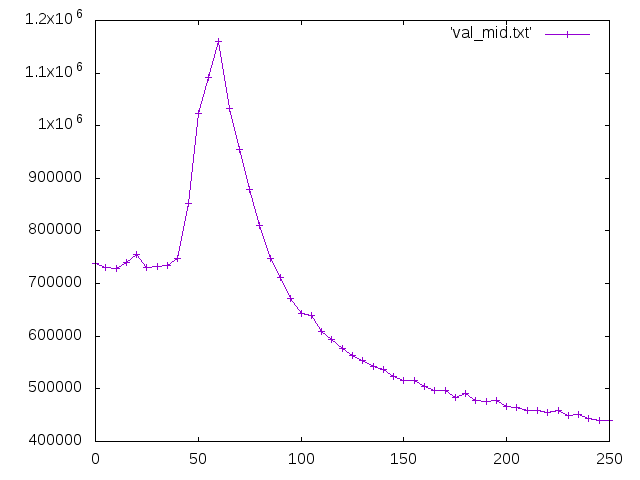
\includegraphics[width=2in]{midplot}
	\end{center}
	\caption{Inefficient hill climbing}
	\label{f:midplot}
\end{figure}

To verify that hill climbing is not efficient, we pick one of the earlier groups of photos as an example.
The focus function values for different focus positions are shown in Figure~\ref{f:midplot}.
Let us go through this group of photos according to hill climbing method.
Here we list them in sequence with both the focus position and the focus function value.

Step of 50: 250(440698), 200(466670), 150(516504), 100(644100), 50(1022550), 0(738123, getting smaller, reverse)

Step of 10: 10(728320), 20(755560), 30(732839), 40(748476), 50(1022550), 60(1159197), 70(955419, getting smaller, reverse)

Step of 5: 65(1032810), 60(1159197), 55(1092617, getting smaller, 5 is minimum step, stop at 60)

We can see that the global optimum is at focus position 60.
However, at the step of 50, the value did not get smaller, so focus actually goes to 0 first then gradually upwards via 10, 20, ...
This shows that this is different from normal binary search, and this one more step results in 6 more photos captured and 6 more focus function calculated.
Remember that hill climbing does not have additional memory so every time the value needs to be recalculated over and over again.

Just imagine, if we do the experiment under Windows where minimum step of 1 is supported, it could result in much much longer time of the focus process.

For \sysname, the details are shown below.
In Figure~\ref{f:param}, we can see that the focus position ranges from 0 to 250 and the minimum step is 5.
There are 2 versions of \sysname, where v1 has the step of 25 and v2 has the step of 50.
In other words, v1 takes photos only at the focus position of 0, 25, 50, 75, 100, 125, 150, 175, 200, 225 and 250, which includes 11 photos.
Similarly, v2 takes photos only at the focus position of 0, 50, 100, 150, 200, 250.

To evaluate our method, we also implement our version of hill climbing.
We implement hill climbing with the initial step of 50, then drops to 10 and finally to 5.
The initial position of focus is 250, which is the closest position from the camera sensor and has the clearest view of close objects.
When the process starts, it moves towards 0 and then switch when the focus function gets smaller.

To make the time of photo capturing more accurate, we take the photos at all focus positions (every 5 millimeters) in advance so that we can ignore the hardware time difference caused by the whole system.

We first tried ffmpeg as the photo capturing tool, but the time the process takes is just too long.
Taking one shot is over 1.5 seconds and that is not reasonable.
Now we use VideoCapture library in Python and it works perfectly.

The Laplacian operator is applied to every pixel of the photos and we use Python library as the implementation.
This could lead to slower process but as long as we use the same focus function implementation in the both hill climbing and \sysname, the results are still convincing.

\section{Evaluation}

\begin{figure}[tb!]
	\begin{center}
		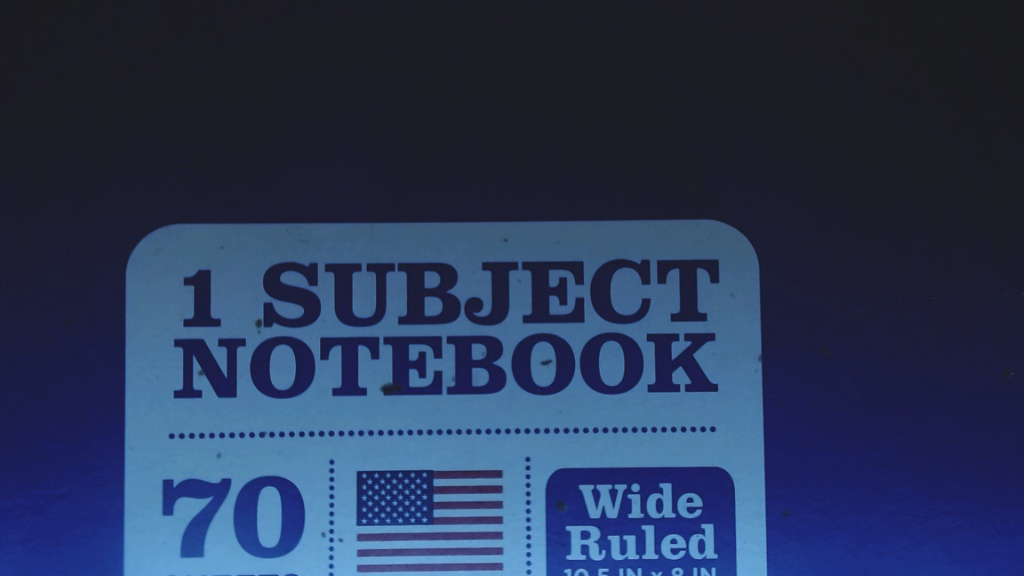
\includegraphics[width=2in]{noteclose}
	\end{center}
	\caption{Optimal focused noteclose (u=5cm,focus=125,val=812824)}
	\label{f:noteclose}
\end{figure}

\begin{figure}[tb!]
	\begin{center}
		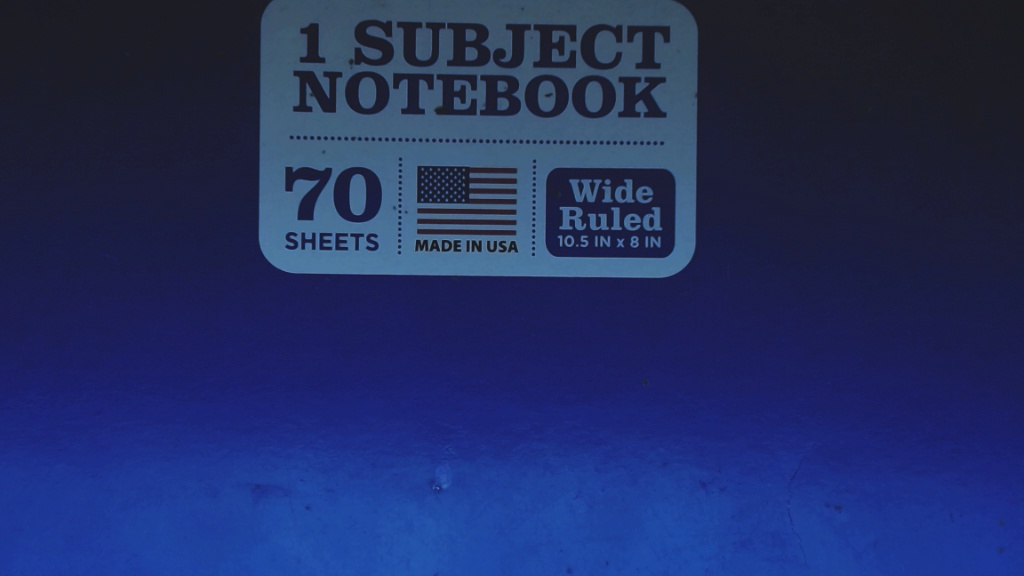
\includegraphics[width=2in]{notebook}
	\end{center}
	\caption{Optimal focused notebook (u=10cm,focus=80,val=692750)}
	\label{f:notebook}
\end{figure}

\begin{figure}[tb!]
	\begin{center}
		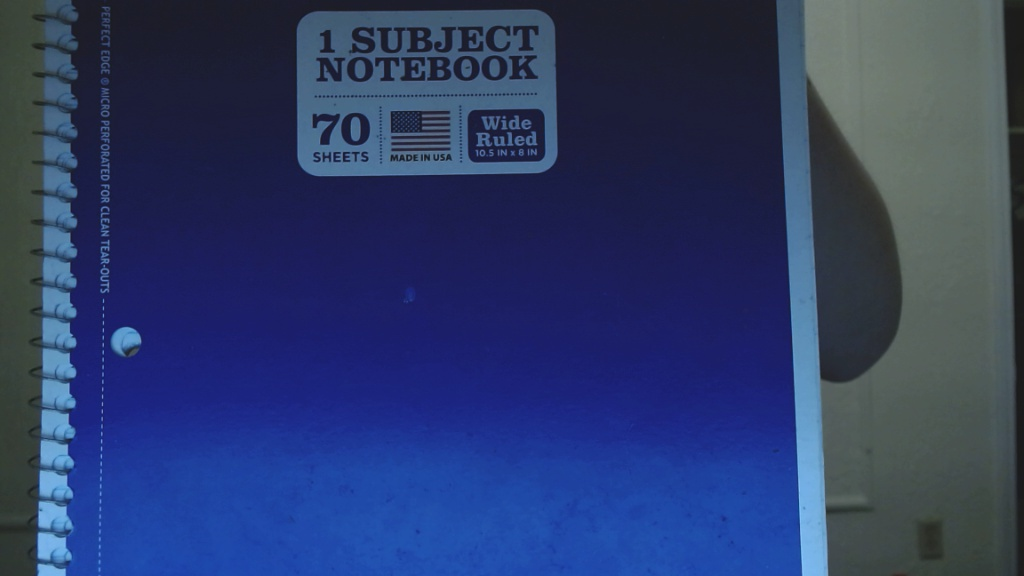
\includegraphics[width=2in]{notemid}
	\end{center}
	\caption{Optimal focused notemid (u=20cm,focus=125,val=812824)}
	\label{f:notemid}
\end{figure}

\begin{figure}[tb!]
	\begin{center}
		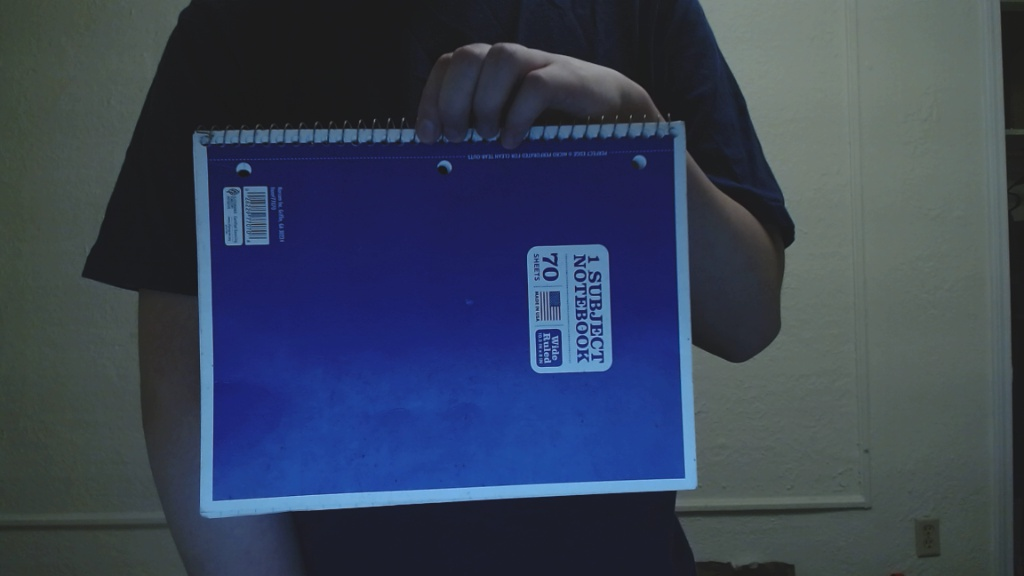
\includegraphics[width=2in]{notefar}
	\end{center}
	\caption{Optimal focused notefar (u=40cm,focus=125,val=812824)}
	\label{f:notefar}
\end{figure}

\begin{figure}[tb!]
	\begin{center}
		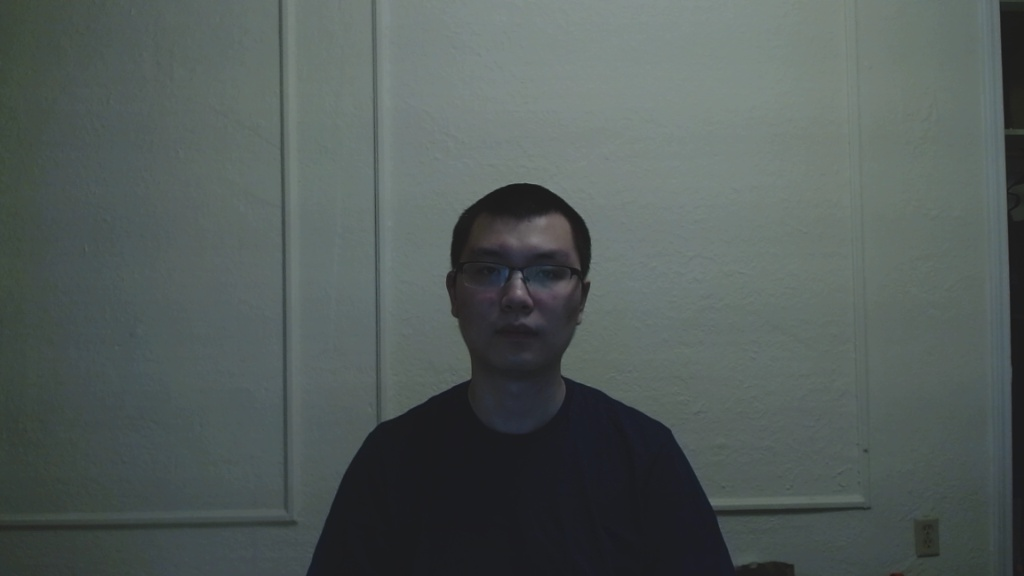
\includegraphics[width=2in]{human}
	\end{center}
	\caption{Optimal focused human (u=1m,focus=125,val=812824)}
	\label{f:human}
\end{figure}

We collect 5 groups of photos, with the object distance from closer to further.
We name the photos as noteclose(Figure~\ref{f:noteclose}), notebook(Figure~\ref{f:notebook}), notemid(Figure~\ref{f:notemid}), notefar(Figure~\ref{f:notefar}), human(Figure~\ref{f:human}) with the distance of 5cm, 10cm, 20cm, 40cm and 1m respectively.
Photos at all focus positions (with 5mm minimum step) are collected in advance and during the evaluation process, the camera is turned on but no photo is collected.
We use the photos collected ahead of time.

\begin{figure}[tb!]
	\begin{center}
		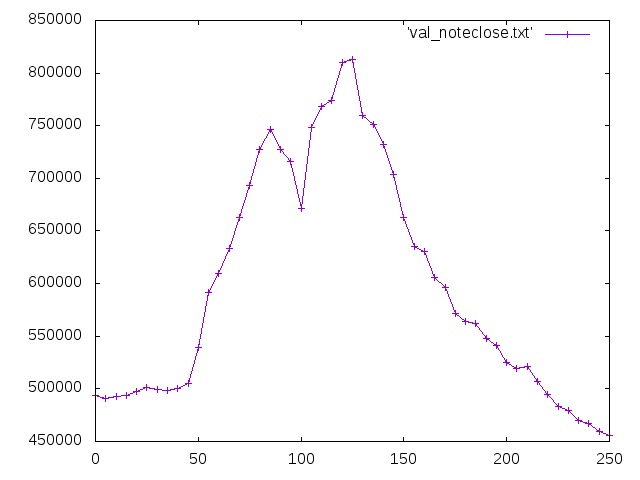
\includegraphics[width=2in]{notecloseplot}
	\end{center}
	\caption{Noteclose: Focus function values under different focus positions}
	\label{f:notecloseplot}
\end{figure}

\begin{figure}[tb!]
	\begin{center}
		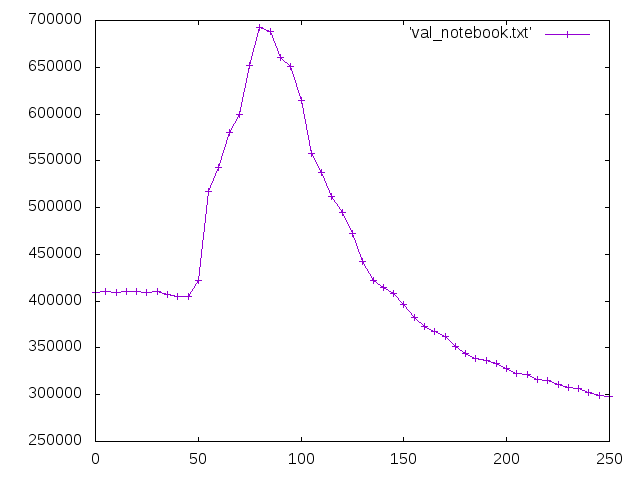
\includegraphics[width=2in]{notebookplot}
	\end{center}
	\caption{Notebook: Focus function values under different focus positions}
	\label{f:notebookplot}
\end{figure}
\begin{figure}[tb!]
	\begin{center}
		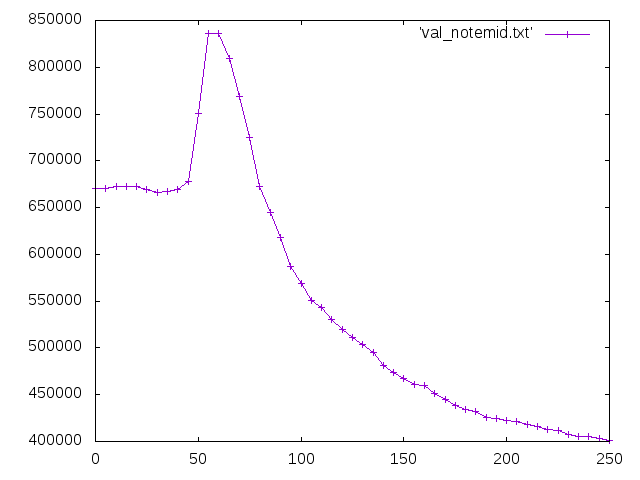
\includegraphics[width=2in]{notemidplot}
	\end{center}
	\caption{Notemid: Focus function values under different focus positions}
	\label{f:notemidplot}
\end{figure}
\begin{figure}[tb!]
	\begin{center}
		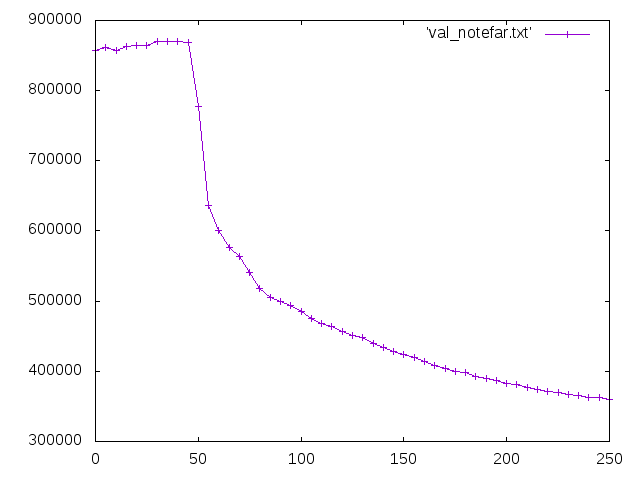
\includegraphics[width=2in]{notefarplot}
	\end{center}
	\caption{Notefar: Focus function values under different focus positions}
	\label{f:notefarplot}
\end{figure}
\begin{figure}[tb!]
	\begin{center}
		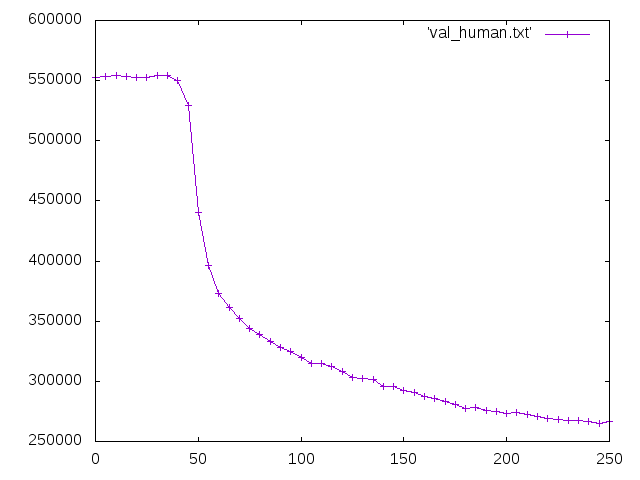
\includegraphics[width=2in]{humanplot}
	\end{center}
	\caption{Human: Focus function values under different focus positions}
	\label{f:humanplot}
\end{figure}

Figure~\ref{f:notecloseplot}, Figure~\ref{f:notebookplot}, Figure~\ref{f:notemidplot}, Figure~\ref{f:notefarplot}, Figure~\ref{f:humanplot} show the focus function values when lens are at different positions.
You may notice that in general, these curves contain only 1 ``hill''.
There are some jitters causing some local maximum appearing.
If there is only 1 ``hill'' in a curve, then the naive hill climbing should be able to reach the global maximum.

\begin{table} [tb!]\tiny
	\centering
	\begin{tabular} {| c | c | c | c | c | c |}
		\hline
		focus/val & \textbf{Noteclose} & \textbf{Notebook} & \textbf{Notemid} & \textbf{Notefar} & \textbf{Human} \\
		\hline
		Optimal(Ground Truth) & 125/812824 & 80/692750 & 60/836247 & 35/870166 & 35/554606 \\
		\hline
		HillClimbing & 85/746181 & 80/692750 & 15/672973 & 5/862217 & 10/554338 \\
		\hline
		\sysname v1 & 125/812824 & 75/652280 & 50/750514 & 25/864501 & 25/552651\\
		\hline
		\sysname v2 & 100/671497 & 100/614299 & 50/750514 & 0/857793 & 0/552585\\
		\hline
	\end{tabular}
	\caption{Focus position and function values of results using different method}
	\label{t:r1}
\end{table}

In Table~\ref{t:r1}, we can see that HillClimbing falls into local maximum in 4 out of 5 cases.
In general, the result function value is not too far away from the ground truth.
But if we combine the results from Table~\ref{t:r2}, we can see that the time of focusing is strongly decided by the number of photos taken.

Next, let us compare v1 and v2 of \sysname.
In Table~\ref{t:r1}, it is obvious that v1 has more accurate results than v2, which means better-focused outcome photos.
However if we take a look at Table~\ref{t:r2}, we can see that the time used by v2 is much shorter than v1, almost halved.
Thus we know that v1 and v2 is a tradeoff between the accuracy and the speed.
\sysname has a more stable focusing time once the step is decided.
Larger step means faster focusing speed and smaller step means better-focused photos.

In Table~\ref{t:r1}, v1 has similar processing time with HillClimbing, but from Table~\ref{t:r1}, surprisingly we see that the focus effect is slightly better than HillClimbing.

\begin{table} [tb!]\scriptsize
	\centering
	\begin{tabular} {| c | c | c | c | c | c |}
		\hline
		Time(s) & \textbf{Noteclose} & \textbf{Notebook} & \textbf{Notemid} & \textbf{Notefar} & \textbf{Human} \\
		\hline
		HillClimbing & 5.71 & 5.07 & 4.29 & 4.16 & 4.69 \\
		\hline
		\sysname v1 & 4.89 & 4.64 & 4.79 & 4.68 & 4.63\\
		\hline
		\sysname v2 & 2.84 & 2.93 & 2.86 & 2.87 & 2.92\\
		\hline
	\end{tabular}
	\caption{Time used on focusing for different groups of photos}
	\label{t:r2}
\end{table}

In Table~\ref{t:r2}, we can see that \sysname v2 greatly speed up the focusing process.
In the best case the speed boost is 50.3\% and on average it is 39.7\% faster.
This is a huge improvement under most cases.

Surely from Table~\ref{t:r1} we can see the quality loss of the picture, in noteclose case it is the worst which is 18\% when evaluated by focus function.
On average, it is a 8.1\$ loss.

To give people a better understanding about the loss, we show you the worst case result provided by \sysname v2 in Figure~\ref{f:worst}.
Compared with Figure!\ref{f:noteclose}, it is not bad at all.

\begin{figure}[tb!]
	\begin{center}
		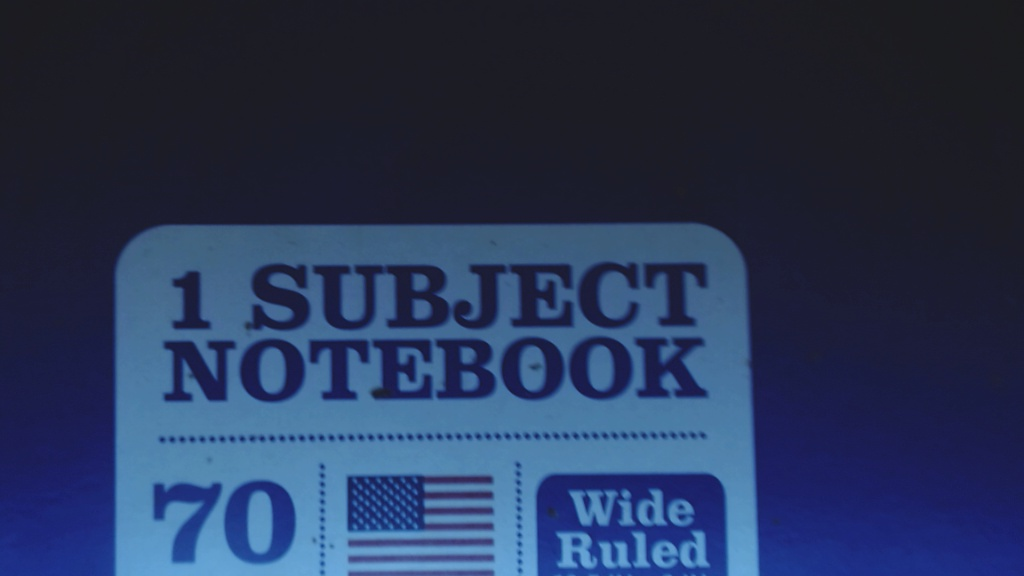
\includegraphics[width=2in]{worst}
	\end{center}
	\caption{Worst case blurry for noteclose}
	\label{f:worst}
\end{figure}


\section{Discussions}

\textbf{Difference of applied scenes:}
All of our experiements are executed using Logitech C920 camera, which is a desktop camera for video calls so the range is used for a person sitting in front of a computer.
However, our potential use case is for phone taking photos.
Phone cameras obviously have larger range, especially a much further distance.

\textbf{Focus function:}
The current focus function is still very inefficient.
Nowadays cameras tend to only includes a few sampling pixels to calculate the derivative sum.
These samples usually are in the central area of the photos.
This way the calculation of focus functions are greatly speeded up.

\textbf{Minimum step of focus position:}
Currently all the experiments are done under Linux, where minimal step of 5mm is supported by UVC cameras under Linux.
If we move the experiments to Windows where 1mm is supported, that indicates 5 more captures on average for a single photo, which further extends the speedup effect of \sysname.

\textbf{Hardware time:}
The scripts and codes in this experiment produce ridiculously long focusing time, which lasts seconds.
This is caused by the software implementation.
In real cameras, all the steps mentioned are implemented in hardware, which should be hundreds of times faster.

\begin{figure}[tb!]
	\begin{center}
		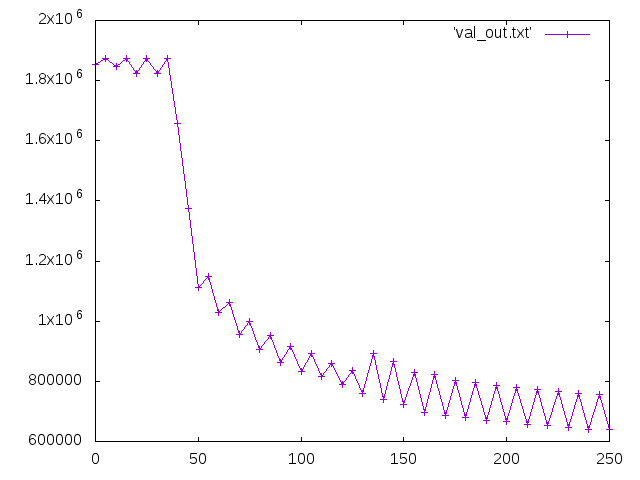
\includegraphics[width=2in]{outplot}
	\end{center}
	\caption{Wave effect caused by exposure time}
	\label{f:outplot}
\end{figure}

\textbf{Exposure, white balance play important parts:}
In Figure~\ref{f:outplot}, we present the function value results when we have auto exposure time enabled.
The photo is the same as human, and the function value is shown in Figure~\ref{f:humanplot}.
We can see that the general pattern is similar but the wave effect exists when auto exposure is enabled.
With auto exposure, the brightness and contrast of the figure is greatly impacted so we need to fix these third-party parameters to ensure stablized curve.

\section{Applications}

Combined with the VR store visit project, \sysname provides better support for data collection.
It reduces the time when visitors need to take photos from stores.
With the cheap devices we already own, it greatly improves the quality of the photos instead of using videos from cheap sport cameras.

When we need to take a large amount of photos, \sysname greatly speed up the whole process.
In some special scenarios, when the object distance is relatively fixed, \sysname can be better applied while not using mechanice in the default hardware.
Cases include street view from the cross, store shelves photographing and museum virtual visits.
In these scenarios, \sysname helps a lot.


\clearpage
\bibliographystyle{plain}
\bibliography{reference}

\end{document}
\grid
